\documentclass{article}
\usepackage{tikz}

\begin{document}

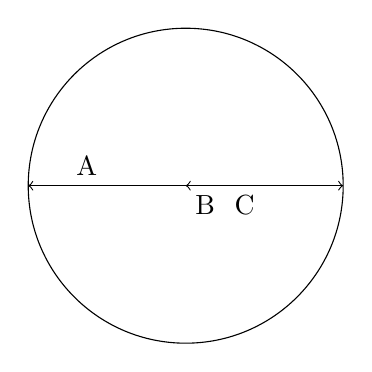
\begin{tikzpicture}
    % Draw the circle
    \draw (0,0) circle (2cm);
    
    % Draw the arcs with labels
    \draw[->] (0,0) -- node[midway, above left] {A} (180:2cm); % Arc from 0 to 180 degrees
    \draw[->] (180:2cm) -- node[midway, below right] {B} (360:2cm); % Arc from 180 to 360 degrees
    \draw[->] (360:2cm) -- node[midway, below left] {C} (0,0); % Arc from 360 to 0 degrees
    
    % Draw additional points or lines as needed
\end{tikzpicture}

\end{document}